\usepackage{movie15}
\documentclass{beamer}
%
% Choose how your presentation looks.
%
% For more themes, color themes and font themes, see:
% http://deic.uab.es/~iblanes/beamer_gallery/index_by_theme.html
%
\mode<presentation>
{
  \usetheme{Warsaw}      % or try Darmstadt, Madrid, Warsaw, ...
  \usecolortheme{default} % or try albatross, beaver, crane, ...
  \usefonttheme{default}  % or try serif, structurebold, ...
  \setbeamertemplate{navigation symbols}{}
  \setbeamertemplate{caption}[numbered]
  
  \addtobeamertemplate{navigation symbols}{}{%
    \usebeamerfont{footline}%
    \usebeamercolor[fg=blue]{footline}%
    \hspace{1em}%
    \insertframenumber/\inserttotalframenumber
}
} 

\usepackage[english]{babel}
\usepackage[utf8x]{inputenc}

\title[CNN, RNN \& LSTM]{CNN, RNN \& LSTM}
\author{Himanshu Singh}
\institute{IIT Bombay}
\date{}

\begin{document}

\begin{frame}
  \titlepage
\end{frame}

% Uncomment these lines for an automatically generated outline.
%\begin{frame}{Outline}
%  \tableofcontents
%\end{frame}
\begin{frame}[t]{Convolution}

\only<1>{\begin{figure}
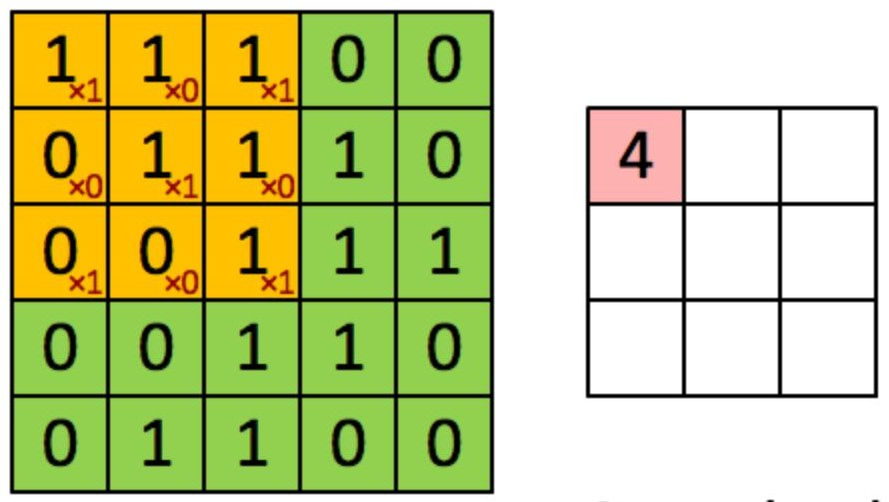
\includegraphics[width=6cm, height=3.25cm]{c1.jpg}
\end{figure}}


\only<2>{\begin{figure}
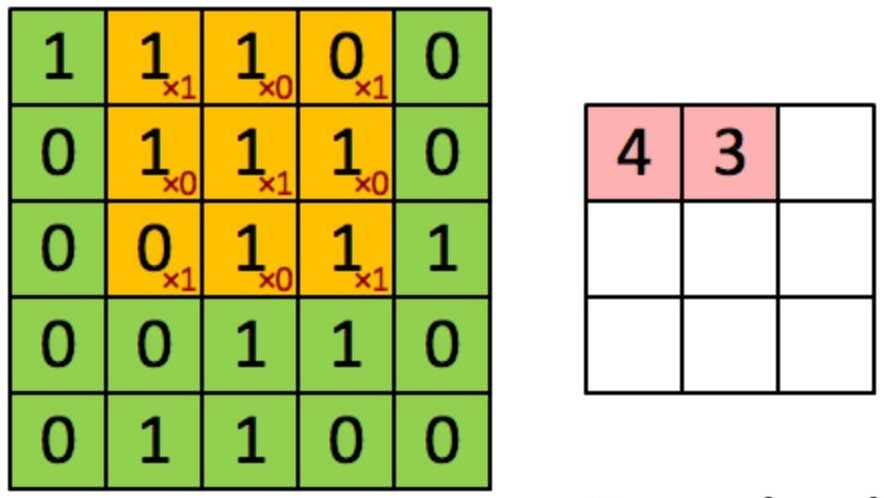
\includegraphics[width=6cm, height=3.25cm]{c2.jpg}
\end{figure}}

\only<3>{\begin{figure}
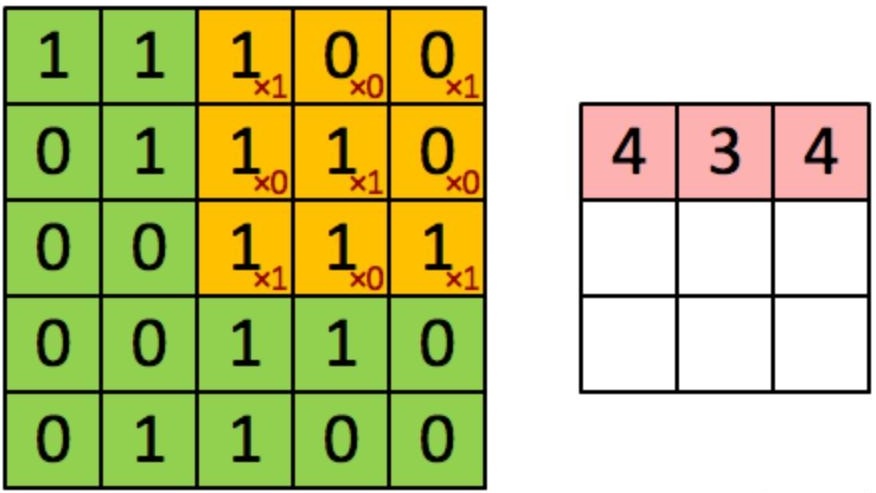
\includegraphics[width=6cm, height=3.25cm]{c3.jpg}
\end{figure}}

\only<4>{\begin{figure}
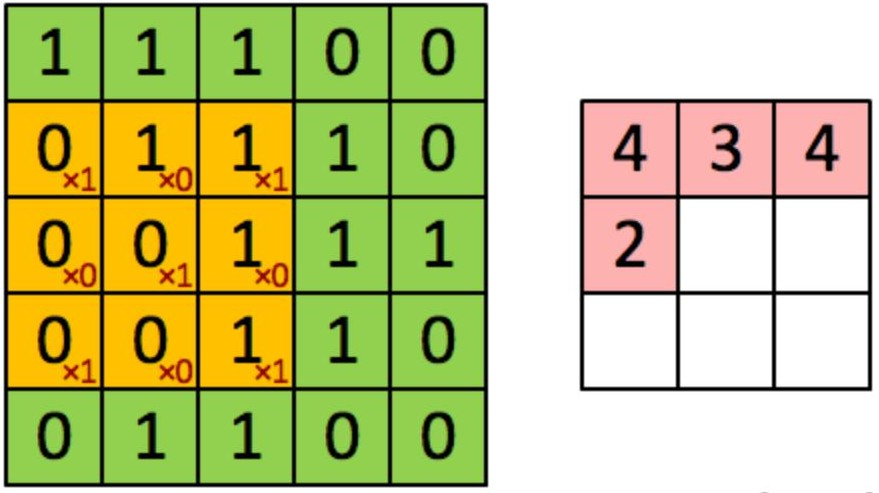
\includegraphics[width=6cm, height=3.25cm]{c4.jpg}
\end{figure}}
    
\only<5>{\begin{figure}
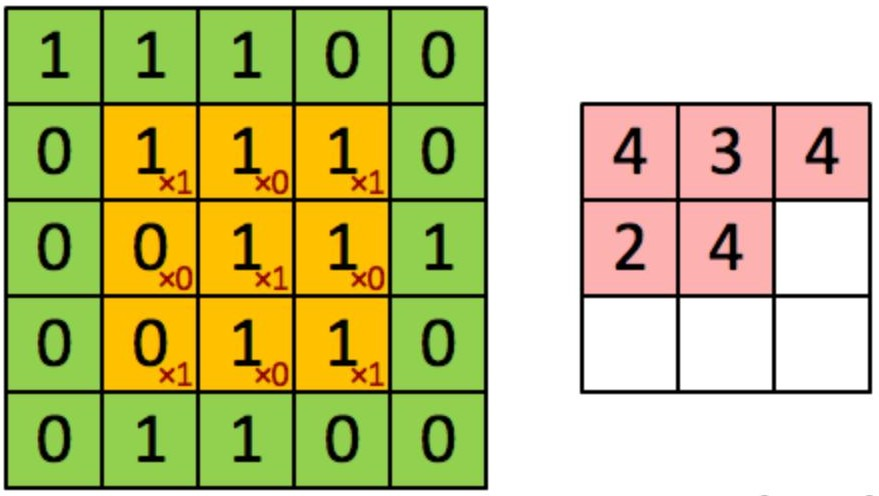
\includegraphics[width=6cm, height=3.25cm]{c5.jpg}
\end{figure}}    

\only<6>{\begin{figure}
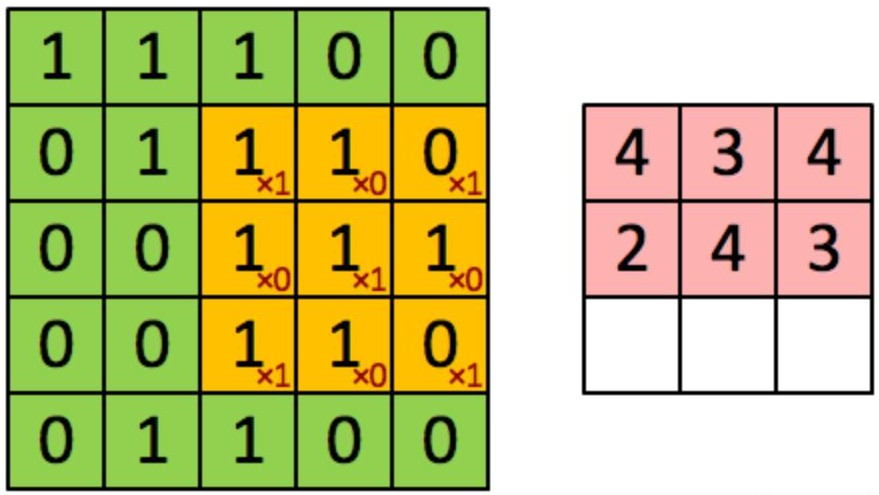
\includegraphics[width=6cm, height=3.25cm]{c6.jpg}
\end{figure}}

\only<7>{\begin{figure}
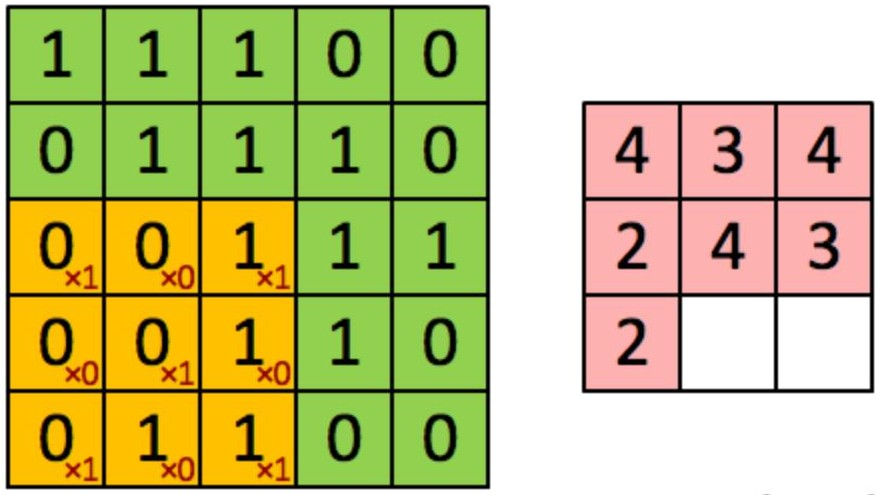
\includegraphics[width=6cm, height=3.25cm]{c7.jpg}
\end{figure}}
    
\only<8>{\begin{figure}
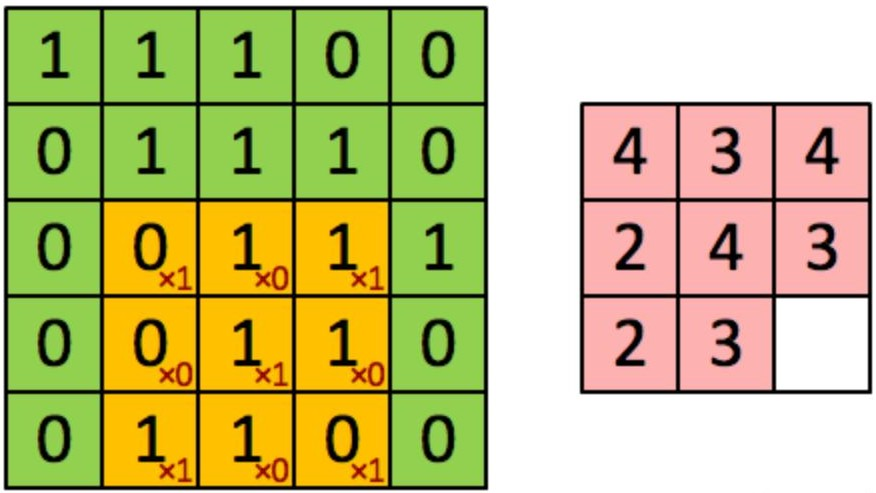
\includegraphics[width=6cm, height=3.25cm]{c8.jpg}
\end{figure}}    
    
\only<9>{\begin{figure}
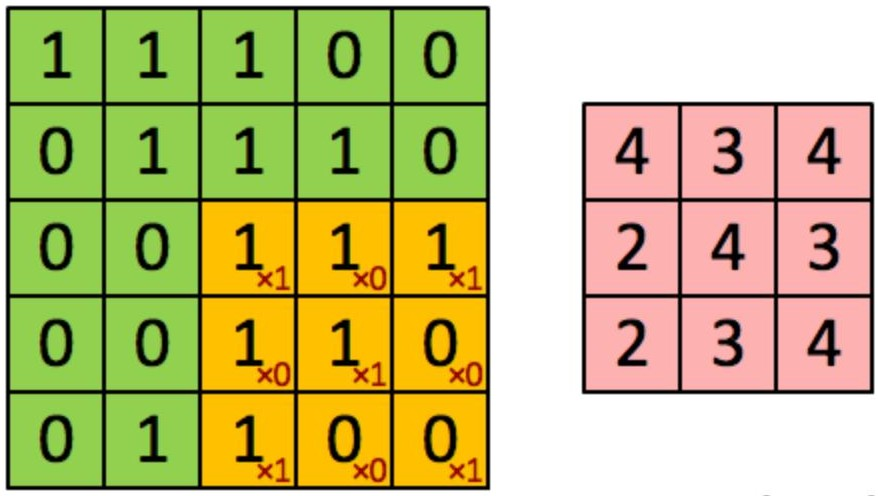
\includegraphics[width=6cm, height=3.25cm]{c9.jpg}
\end{figure}}    
    
\hspace{2cm}\tiny{http://deeplearning.stanford.edu/wiki/index.php/Feature_extraction_using_convolution}
    
\end{frame}


\begin{frame}{Why Convolution?}
Averaging each pixel with its neighboring values blurs an image:
\begin{figure}
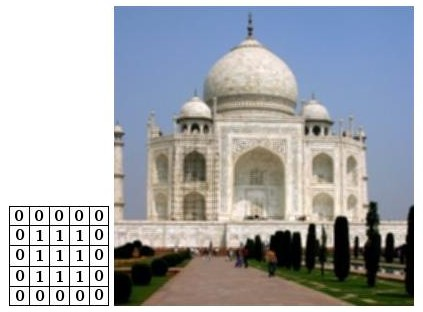
\includegraphics[width=3cm, height=2.25cm]{blur.jpg}
\end{figure}
Taking the difference between a pixel and its neighbors detects edges:
\begin{figure}
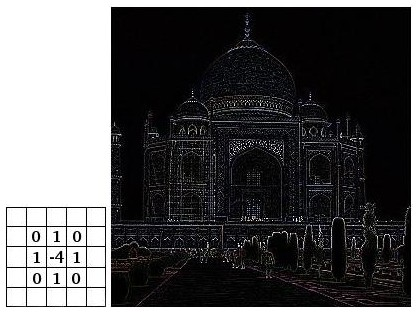
\includegraphics[width=3cm, height=2.25cm]{edges.jpg}
\end{figure}

\hspace{3cm}\tiny{https://docs.gimp.org/en/plug-in-convmatrix.html}
    
\end{frame}

\begin{frame}[t]{What is Convolutional Neural Network?}
\begin{block}{CNN}
It is several layers of convolutions with nonlinear activation functions like ReLU or tanh applied to the results
\end{block}
\begin{itemize}
    \item During the training phase, a CNN automatically learns the values of its filters based on the task you want to perform.
    \item \textbf{Location Invariance :} Let’s say you want to classify whether or not there’s an elephant in an image. Because you are sliding your filters over the whole image you don’t really care where the elephant occurs.
    
    \item \textbf{Compositionality :} Each filter composes a local patch of lower-level features into higher-level representation. 
\end{itemize}
    
\end{frame}

\begin{frame}{What has CNN for NLP?}

\begin{figure}
    \centering
    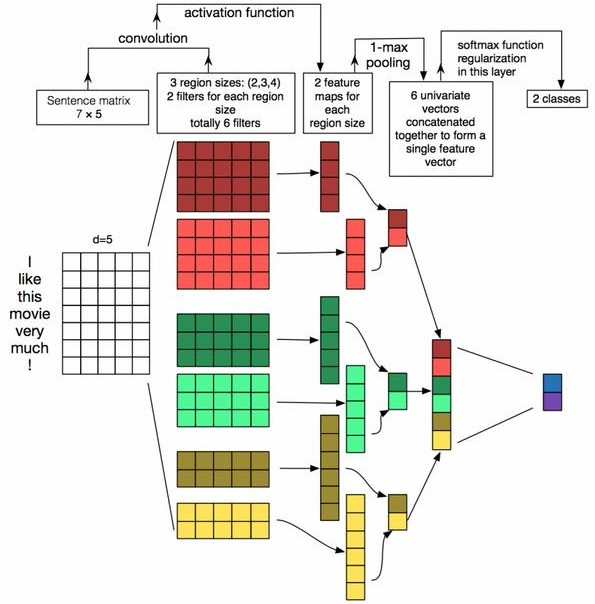
\includegraphics[width=6cm, height=6cm]{cnn_nlp.jpg}
\end{figure}
    \tiny{Zhang, Y., & Wallace, B. (2015). A Sensitivity Analysis of (and Practitioners’ Guide to) Convolutional Neural Networks for Sentence Classification.}
\end{frame}

\begin{frame}{Problems with CNN}
\begin{itemize}
    \item \textbf{Location Invariance} : You probably do care a lot where in the sentence a word appears unlike images.
    
    \item \textbf{Local Compositionality} : Pixels close to each other are likely to be semantically related (part of the same object), but the same isn’t always true for words. In many languages, parts of phrases could be separated by several other words.
    
    \item \textbf{Compositional aspect is intuitive in Computer Vision} i.e. edges form shapes and shapes form objects. Clearly, words compose in some ways, like an adjective modifying a noun, but how exactly this works what higher level representations actually “mean” isn’t as obvious as in the Computer Vision case.
\end{itemize}
\end{frame}


\begin{frame}{Why not a traditional neural network for sequential task?}
\begin{figure}
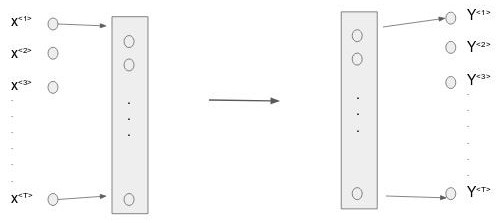
\includegraphics[width=6cm, height=3cm]{feedForwardNN.jpg}
\end{figure}
Problems:
\begin{itemize}
  \item Inputs and ouputs can be of different lengths in different examples
  \item Traditional NN doesn't share features learned accross different positions of text
\end{itemize}
\begin{block}{Recurrent Neural Network}
RNN solves above two problems along with the problems posed by CNNs.
\end{block}
\end{frame}

\begin{frame}[t]{An Unrolled RNN}
NOTE : Hidden state ($h_t$) tells us summary of the sequence till time t
\begin{figure}
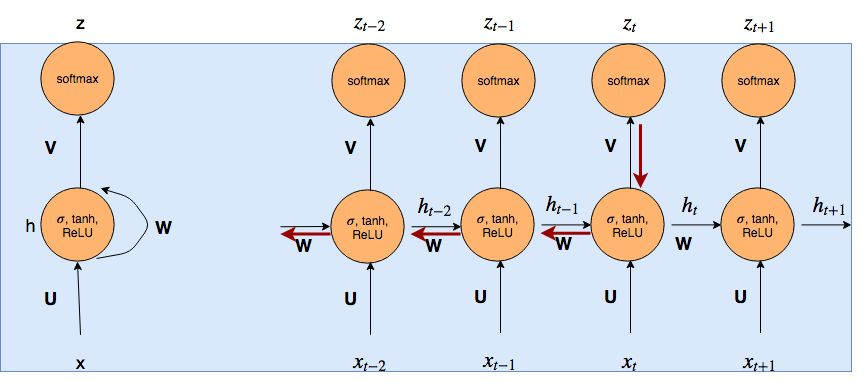
\includegraphics[width=9cm, height=4cm]{unrolled_rnn_1.jpg}
\end{figure}
Forward pass\\
h_t = tanh(Wh_{t-1} + Ux_t + b_h)\\
z_t = softmax(Vh_t + b_z) \\

\end{frame}

\begin{frame}[t]{Backpropagation in RNN}
Notation: E(x, y) = -\sum_{t}y_tlogz_t\\
E : above objective function (i.e. sum of errors at all time stamps)\\
E(t) : to indicate the output at time t\\
\vspace{0.5cm}
We have, h_t = tanh(Wh_{t-1} + Ux_t + b_h)\\
z_t = softmax(Vh_t + b_z) \\
\vspace{0.5cm}
\textbf{Gradient of E w.r.t V}\\
let $\alpha_t = Vh_t + b_z$ then\\
$\frac{\partial E}{\partial V} = \sum_{t} \frac{\partial E}{\partial \alpha_t} \frac{\partial \alpha_t}{\partial V}$
\\
\vspace{0.5cm}
$\frac{\partial E}{\partial \alpha_t}$ is derivative of softmax function w.r.t it's input $\alpha_t\\
$\frac{\partial E}{\partial \alpha_t} = z_t - y_t$ (cite) and $\frac{\partial \alpha_t}{\partial V} = h_t$\\
\vspace{0.5cm}
\\
$\frac{\partial E}{\partial V} = \sum_{t} (z_t - y_t)h_t$\\

\end{frame}




\begin{frame}[t]{Backpropagation in RNN}
    We have\\
    h_t = tanh(Wh_{t-1} + Ux_t + b_h)\\
    z_t = softmax(Vh_t + b_z) \\
    \vspace*{0.5cm}
    \textbf{Gradient of E w.r.t W}\\
    $\frac{\partial E(t)}{\partial W} = \frac{\partial E(t)}{\partial z_t} \frac{\partial z_t}{\partial W} = \frac{\partial E(t)}{\partial z_t}\frac{\partial z_t}{\partial h_t}\frac{\partial h_t}{\partial W}$\\
    \vspace*{0.5cm}
    from forward pass equations, $h_t$ partially depends on $h_{t-1}$\\
    $\frac{\partial E(t)}{\partial W} =  \frac{\partial E(t)}{\partial z_t}\frac{\partial z_t}{\partial h_t}\frac{\partial h_t}{\partial h_{t-1}}\frac{\partial h_{t-1}}{\partial W}$\\
    \vspace{0.5cm}
    if we keep on substituting $h_{t-1}$ in $h_t$ eqn, we'll see that $h_t$ indirectly depends on $h_{t-2}$, $h_{t-3}$ ...\\
    $\frac{\partial E(t)}{\partial W} =  \sum_{k=1}^{t}\frac{\partial E(t)}{\partial z_t}\frac{\partial z_t}{\partial h_t}\frac{\partial h_t}{\partial h_{k}}\frac{\partial h_{k}}{\partial W}$, and\\
    
    $\frac{\partial E}{\partial W} =  \sum_t\sum_{k=1}^{t}\frac{\partial E(t)}{\partial z_t}\frac{\partial z_t}{\partial h_t}\frac{\partial h_t}{\partial h_{k}}\frac{\partial h_{k}}{\partial W}$
    
\end{frame}



\begin{frame}[t]{Backpropagation in RNN}
    
    We have\\
    h_t = tanh(Wh_{t-1} + Ux_t + b_h)\\
    z_t = softmax(Vh_t + b_z) \\
    \vspace*{0.5cm}
    \textbf{Gradient of E w.r.t U}\\
    We can't consider $h_{t-1}$ as constant when taking partial derivative of $h_t$ w.r.t U because $h_{t-1}$ depends on U i.e. $h_{t-1} = tanh(Wh_{t-2}+Ux_{t-1}+b_h)$
    \\
    \vspace{0.5cm}
    Again, we get a similar form\\
    $\frac{\partial E}{\partial U} =  \sum_t\sum_{k=1}^{t}\frac{\partial E(t)}{\partial z_t}\frac{\partial z_t}{\partial h_t}\frac{\partial h_t}{\partial h_{k}}\frac{\partial h_{k}}{\partial U}$\\
    
    
\end{frame}




\begin{frame}[t]{Problem with RNN}
    Look closely to these equations:\\
     $\frac{\partial E}{\partial W} =  \sum_t\sum_{k=1}^{t}\frac{\partial E(t)}{\partial z_t}\frac{\partial z_t}{\partial h_t}\frac{\partial h_t}{\partial h_{k}}\frac{\partial h_{k}}{\partial W}$\\
     $\frac{\partial E}{\partial U} =  \sum_t\sum_{k=1}^{t}\frac{\partial E(t)}{\partial z_t}\frac{\partial z_t}{\partial h_t}\frac{\partial h_t}{\partial h_{k}}\frac{\partial h_{k}}{\partial U}$\\
     \vspace{0.5cm}
     We find out that $\frac{\partial h_t}{\partial h_{k}}$ is again a chain rule.\\
     $\frac{\partial h_t}{\partial h_{k}} = \frac{\partial h_t}{\partial h_{t-1}}\frac{\partial h_{t-1}}{\partial h_{t-2}}...\frac{\partial h_{k+1}}{\partial h_{k}}$
     \vspace{0.5cm}
     \begin{itemize}
         \item If sequence length is large then there will be more number of terms in the product which will result in vanishing gradient problem or exploding gradient problem depending on whether each individual value is less/greater than 1.
        \item LSTM solves this problem to a large extent.
     \end{itemize}
\end{frame}




\begin{frame}[t]{Long Short Term Memory (LSTM) Network}

% \begin{columns}{\onlytextwidth}
% \column{0.3\textwidth}
\begin{figure}
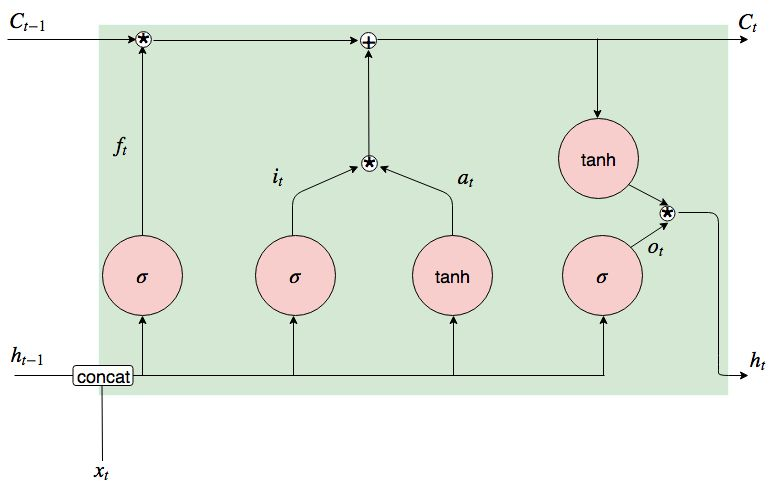
\includegraphics[width=5cm, height=3cm]{lstm.jpg}
% \caption{LSTM node}
\end{figure}
% \column[0.7\textwidth]
Forward Pass\\
f_t = \sigma(W_f[h_{t-1};x_t]+b_f)\\
i_t = \sigma(W_i[h_{t-1};x_t]+b_i)\\
a_t = tanh(W_a[h_{t-1};x_t]+b_a)\\
C_t = f_t*C_{t-1} + i_t*a_t\\
o_t = \sigma(W_o[h_{t-1};x_t]+b_o)\\
h_t = o_t*tanh(C_t)
% \end{columns}

    
\end{frame}

\begin{frame}{Cell state in LSTM}
 
\begin{block}{Vanishing Gradient Problem Addressed}
It runs straight down the entire chain, with only some minor linear interactions. It’s very easy for information to just flow along it unchanged. (Mathematical proof on later slides)
\end{block}

\begin{figure}
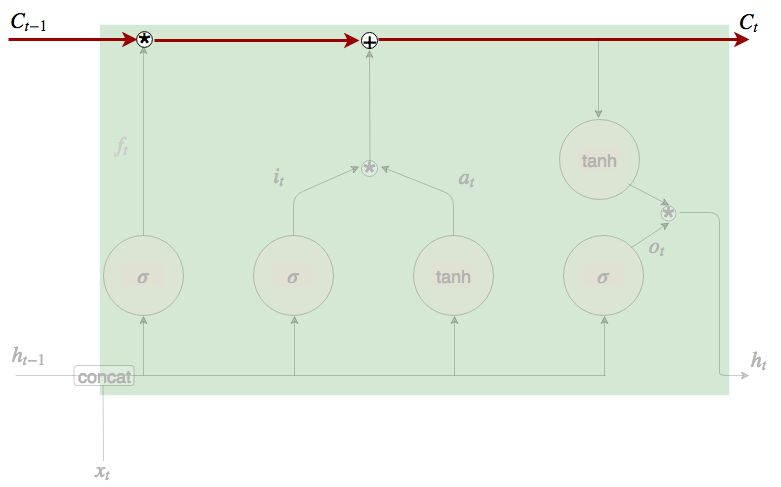
\includegraphics[width=7cm, height=4cm]{lstm_cell_state.jpg}
\end{figure}
\end{frame}


\begin{frame}[t]{Gates in LSTM}
 
\begin{block}{Forget Gate}
Decides what information should be thrown away from the cell state
\end{block}

\begin{figure}
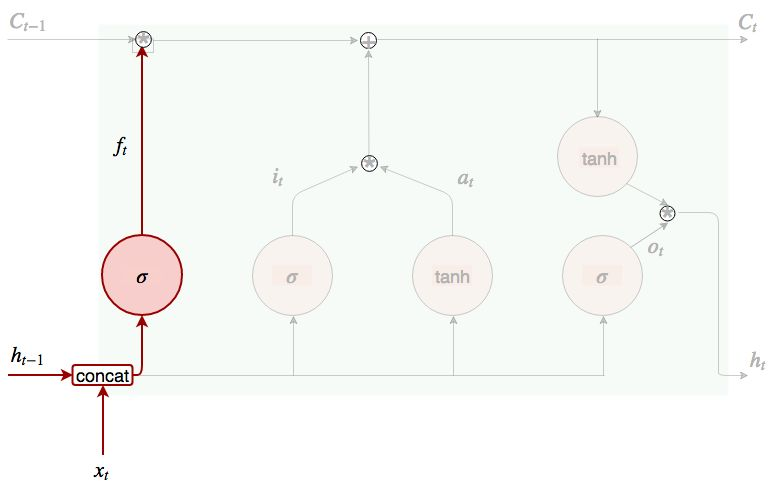
\includegraphics[width=5cm, height=3cm]{forget_gate.jpg}
\end{figure}
    f_t = \sigma(W_f[h_{t-1};x_t]+b_f)\\
\end{frame}

\begin{frame}{Gates in LSTM}
 
\begin{block}{Input Gate}
$\sigma$ layer decides which values to update and $a_t$ is a vector of new candidate values 
\end{block}

\begin{figure}
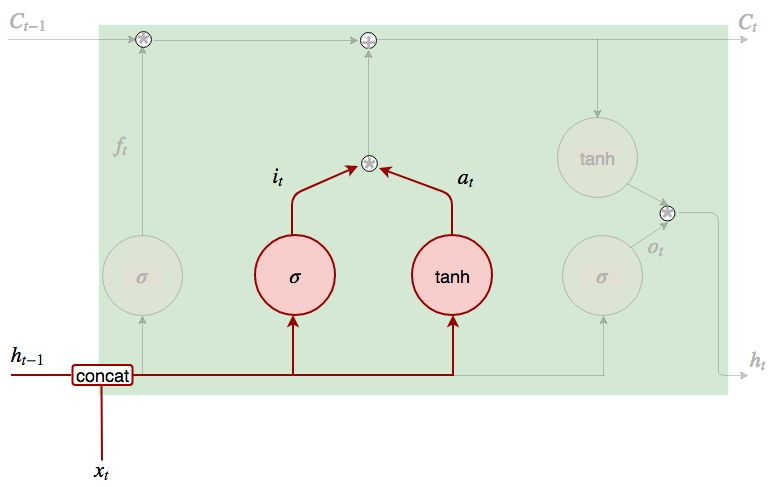
\includegraphics[width=5cm, height=3cm]{input_gate.jpg}
\end{figure}
    i_t = \sigma(W_i[h_{t-1};x_t]+b_i)\\
\end{frame}


\begin{frame}{Gates in LSTM}
 
\begin{block}{Updating Memory Cell}
Multiply the old state by $f_t$, forgetting the things we decided to forget earlier.\\
Then we add $i_t*a_t$. This is the new candidate values, scaled by how much we decided to update each state value.
\end{block}

\begin{figure}
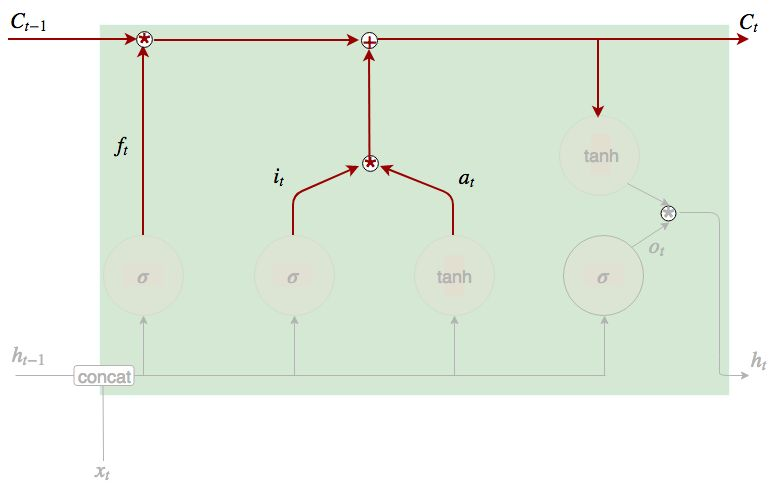
\includegraphics[width=5cm, height=3cm]{lstm_input_modulation.jpg}
\end{figure}
    C_t = f_t*C_{t-1} + i_t*a_t\\
\end{frame}

\begin{frame}{Gates in LSTM}
 
\begin{block}{Output Gate}
Output will be based on our cell state, but will be a filtered version.\\
Cell state is put through tanh to push the output between -1 and 1
\end{block}

\begin{figure}
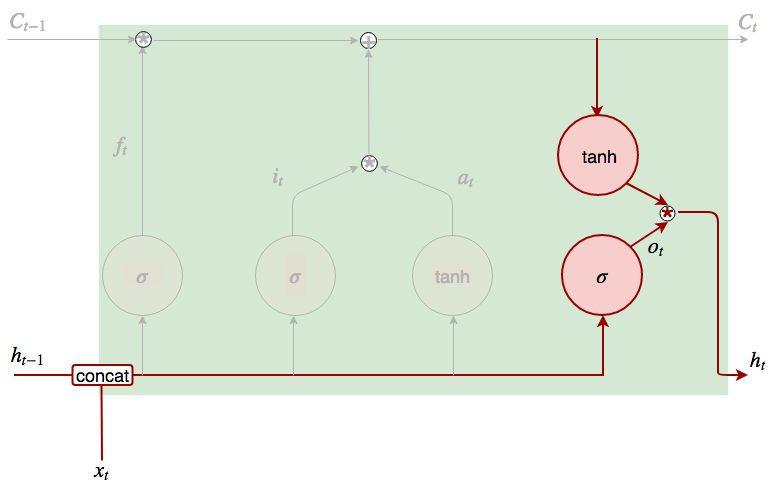
\includegraphics[width=5cm, height=3cm]{lstm_output.jpg}
\end{figure}
    o_t = \sigma(W_o[h_{t-1};x_t]+b_o)\\
    h_t = o_t*tanh(C_t)
\end{frame}


\begin{frame}{Backpropagation in LSTM}
\begin{block}{Error propagation}
Error propagation happens through $C_t$ and $h_t$
\end{block}
\begin{figure}
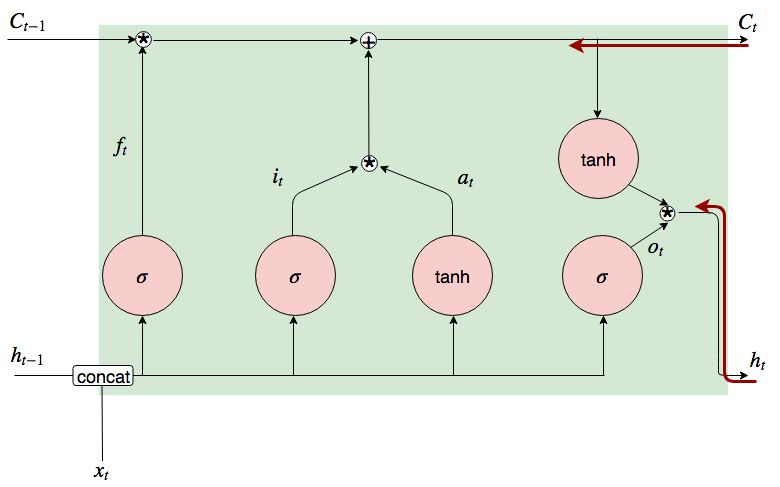
\includegraphics[width=10cm, height=6cm]{lstm_backpropagation.jpg}
\end{figure}
\end{frame}


\begin{frame}{Backpropagation in LSTM}
\begin{block}{Error propagation}
Error propagation through $h_t$
\end{block}

\begin{figure}
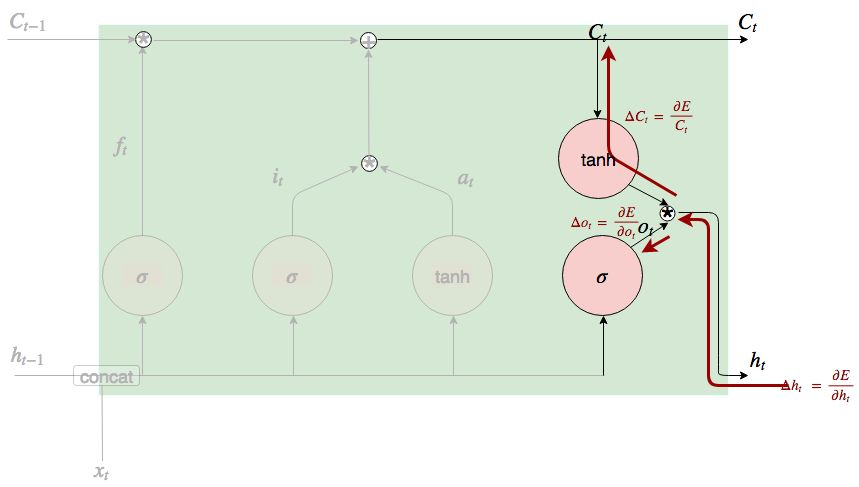
\includegraphics[width=10cm, height=6cm]{lstm_backprop_1.jpg}
\end{figure}
    
\end{frame}

\begin{frame}[t]{Backpropagation in LSTM}
\begin{figure}
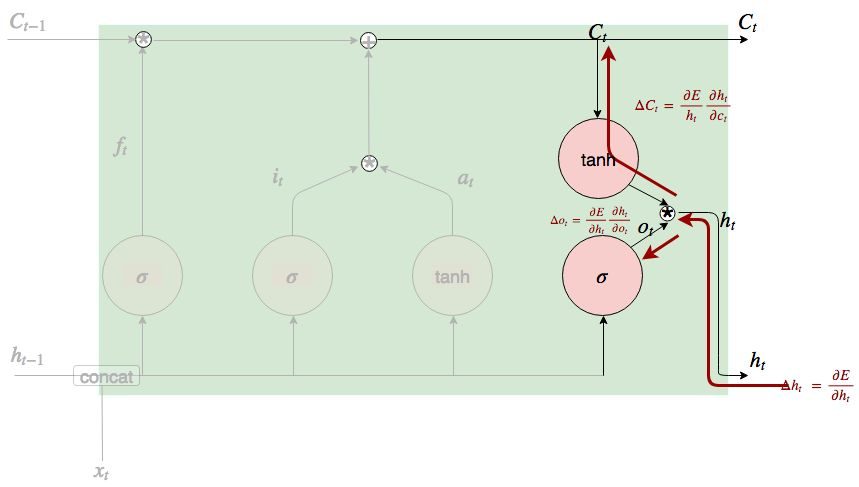
\includegraphics[width=10cm, height=6cm]{lstm_backprop_1_1.jpg}
\end{figure}
o_t = \sigma(W_o[h_{t-1};x_t]+b_o)\\
h_t = o_t*tanh(C_t)\\
\end{frame}

\begin{frame}[t]{Backpropagation in LSTM}
\begin{figure}
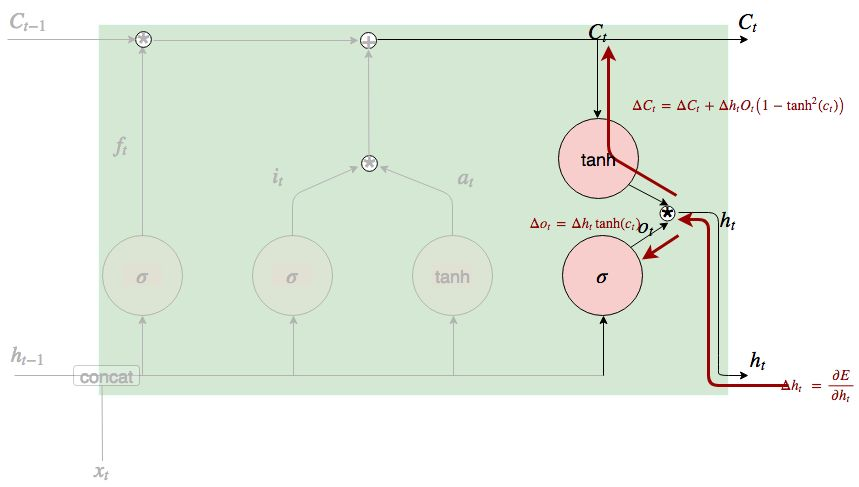
\includegraphics[width=10cm, height=6cm]{lstm_backprop_1_2.jpg}
\end{figure}
    o_t = \sigma(W_o[h_{t-1};x_t]+b_o)\\
    h_t = o_t*tanh(C_t)\\
\end{frame}


\begin{frame}{Backpropagation in LSTM}
\begin{block}{Error propagation}
Error propagation through C_t
\end{block}
\begin{figure}
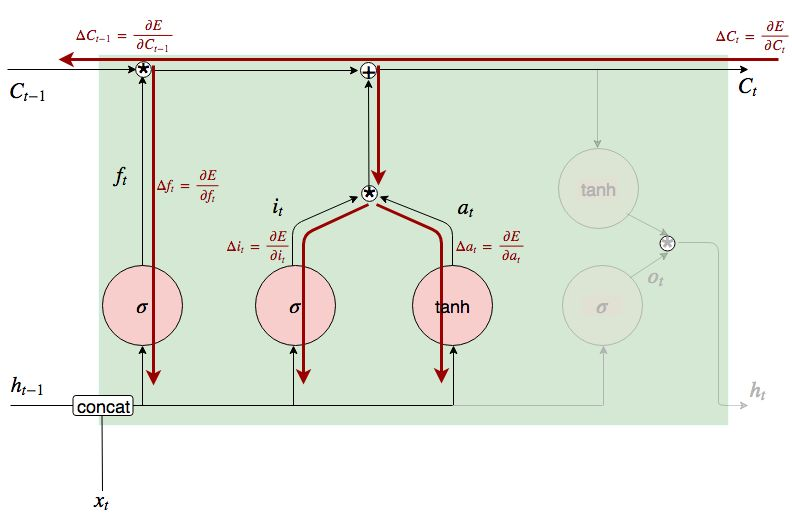
\includegraphics[width=10cm, height=6cm]{lstm_backprop_2.jpg}
\end{figure}
\end{frame}


\begin{frame}{Backpropagation in LSTM}
\begin{figure}
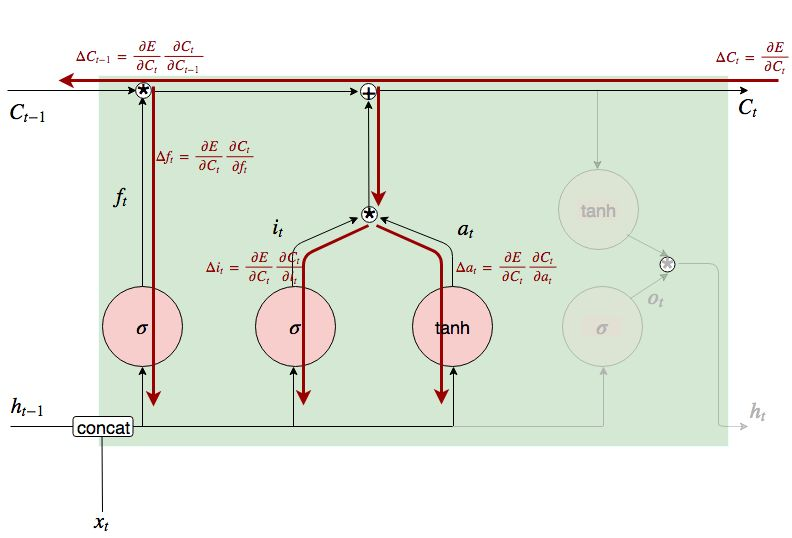
\includegraphics[width=10cm, height=6cm]{lstm_backprop_2_1.jpg}
\end{figure}
C_t = f_t*C_{t-1} + i_t*a_t\\
\end{frame}


\begin{frame}{Backpropagation in LSTM}
NOTE : This $\Delta C_t$ will be used at $(t-1)^{th}$ timestamp for further error propagation. If f is close to 1 then gradient from $t^{th}$ timestamp is propagated perfectly to $(t-1)^{th}$ timestamp.
\begin{figure}
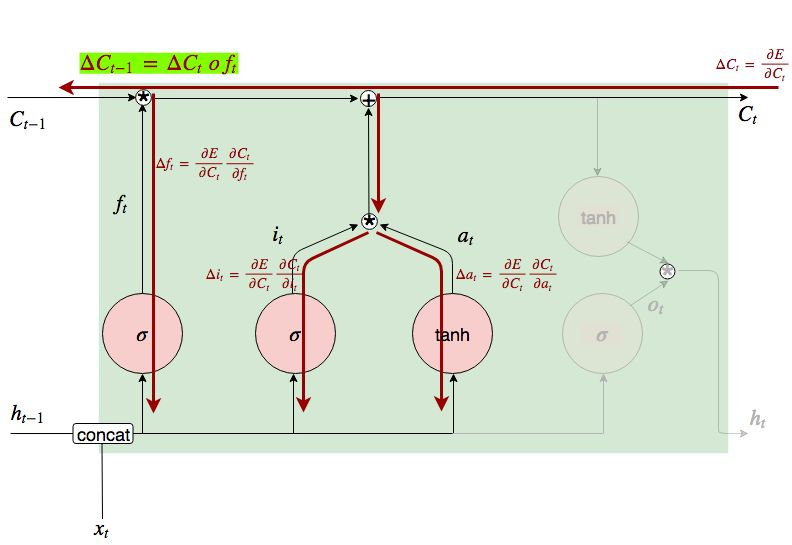
\includegraphics[width=8cm, height=5cm]{lstm_backprop_2_2.jpg}
\end{figure}
C_t = f_t*C_{t-1} + i_t*a_t\\
\end{frame}


\begin{frame}{Backpropagation in LSTM}
\begin{figure}
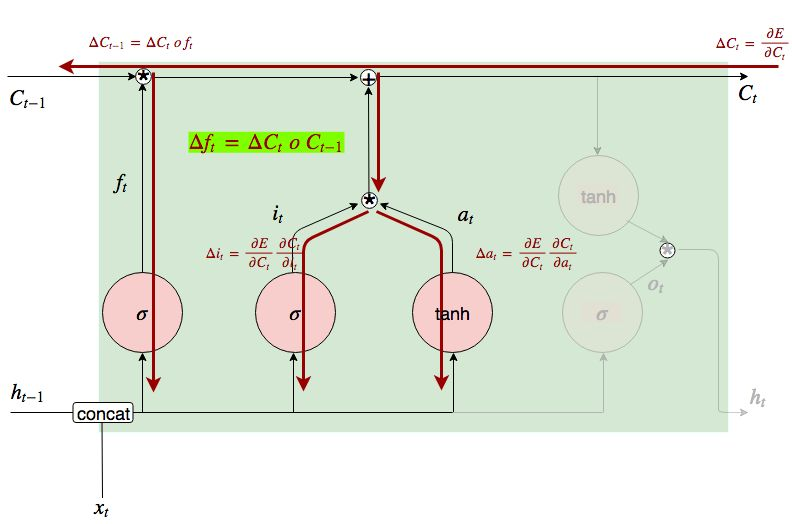
\includegraphics[width=10cm, height=6cm]{lstm_backprop_2_3.jpg}
\end{figure}
C_t = f_t*C_{t-1} + i_t*a_t\\
\end{frame}


\begin{frame}{Backpropagation in LSTM}
\begin{figure}
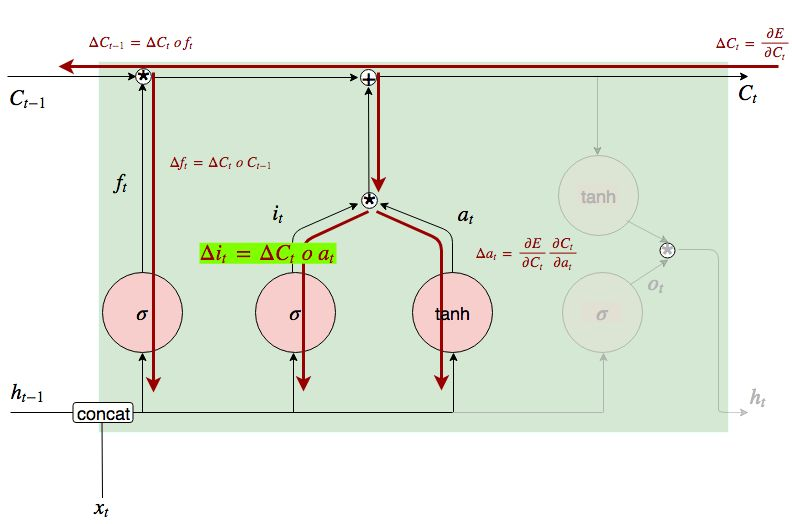
\includegraphics[width=10cm, height=6cm]{lstm_backprop_2_4.jpg}
\end{figure}
C_t = f_t*C_{t-1} + i_t*a_t\\
\end{frame}


\begin{frame}{Backpropagation in LSTM}
\begin{figure}
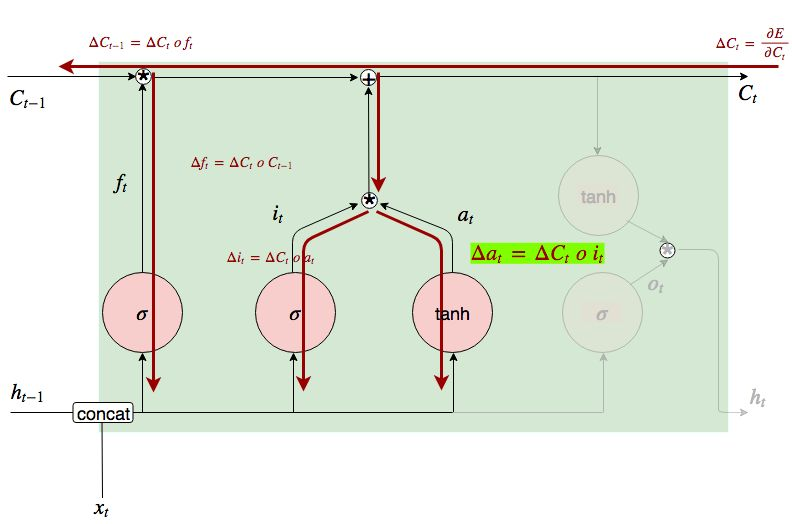
\includegraphics[width=10cm, height=6cm]{lstm_backprop_2_5.jpg}
\end{figure}
C_t = f_t*C_{t-1} + i_t*a_t\\
\end{frame}


\begin{frame}{Backpropagation in LSTM}
\begin{block}{Combined Error}
Error propagation from $C_t$ and $h_t$ both
\end{block}
\begin{figure}
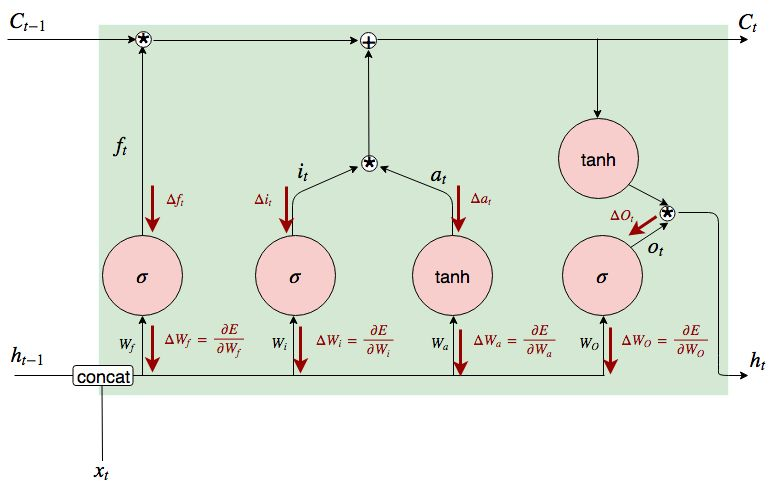
\includegraphics[width=10cm, height=6cm]{lstm_backpropagation_3_1.jpg}
\end{figure}
\end{frame}


\begin{frame}{Backpropagation in LSTM}
\begin{figure}
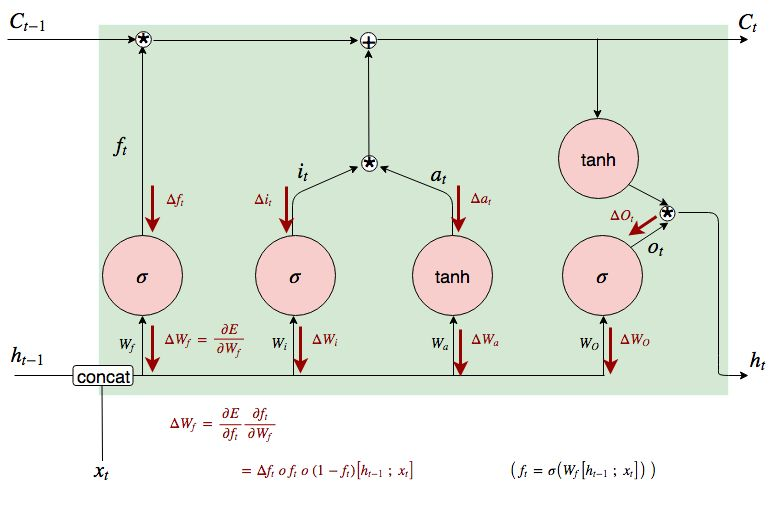
\includegraphics[width=10cm, height=6cm]{lstm_backpropagation_3_2.jpg}
\end{figure}
\end{frame}


\begin{frame}{Backpropagation in LSTM}
\begin{figure}
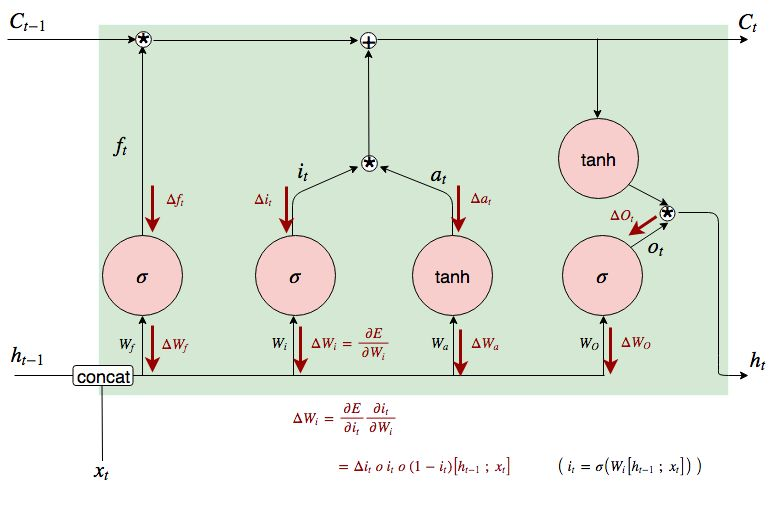
\includegraphics[width=10cm, height=6cm]{lstm_backpropagation_3_3.jpg}
\end{figure}
\end{frame}


\begin{frame}{Backpropagation in LSTM}
\begin{figure}
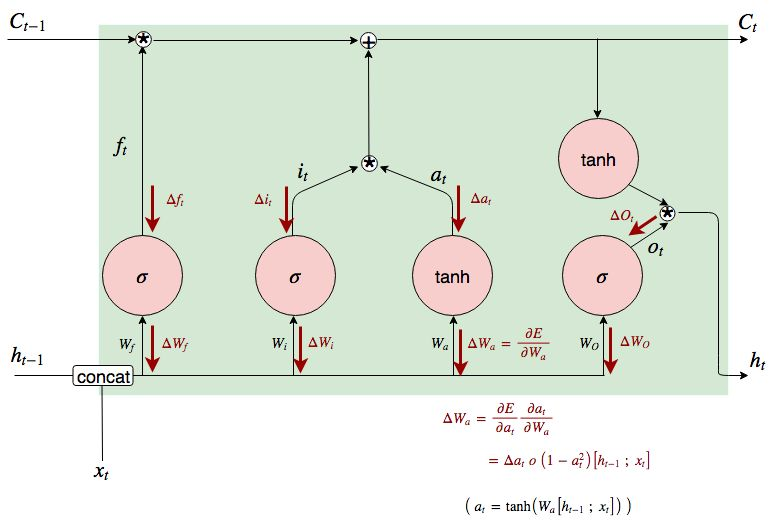
\includegraphics[width=10cm, height=6cm]{lstm_backpropagation_3_4.jpg}
\end{figure}
\end{frame}


\begin{frame}{Backpropagation in LSTM}
\begin{figure}
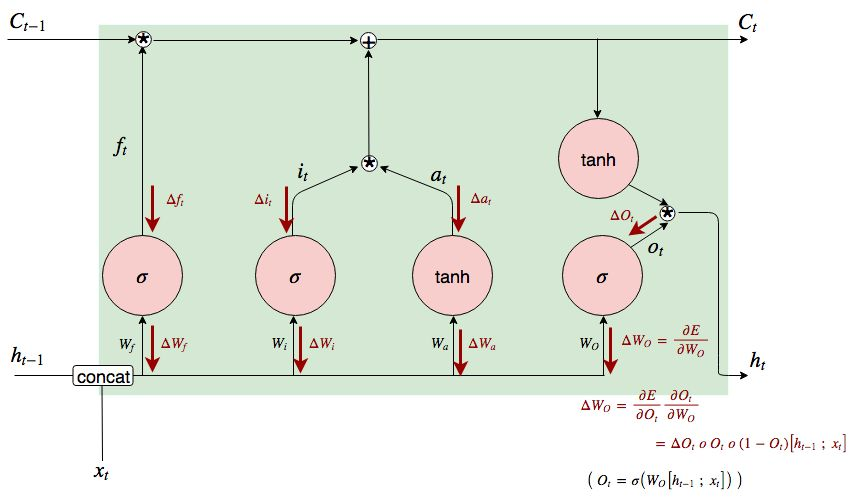
\includegraphics[width=10cm, height=6cm]{lstm_backpropagation_3_5.jpg}
\end{figure}
\end{frame}

\begin{frame}{Backpropagation in LSTM}
\begin{figure}
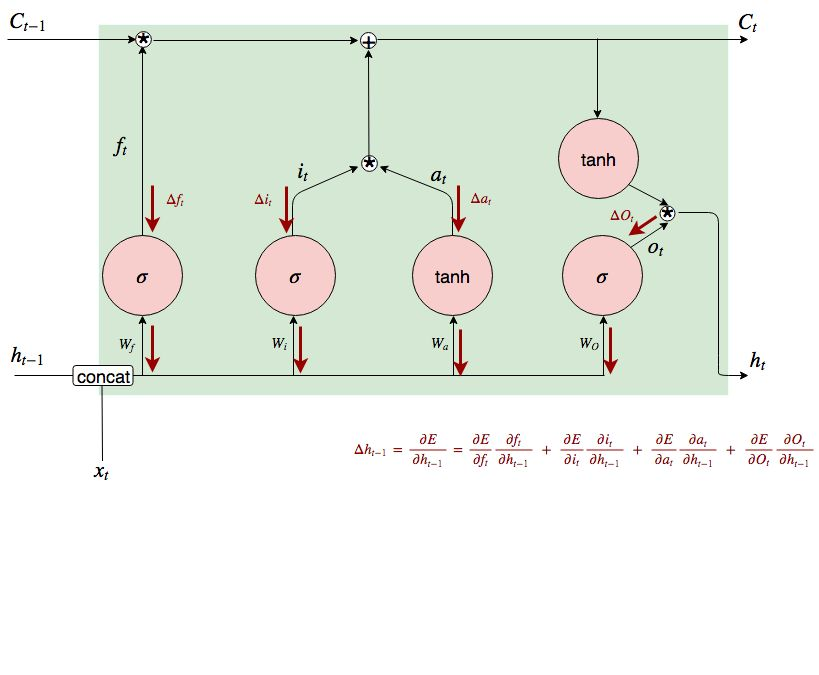
\includegraphics[width=11cm, height=8cm]{lstm_backpropagation_6.jpg}
\end{figure}
\end{frame}


\begin{frame}{Backpropagation in LSTM}
NOTE : $\Delta h_{t-1}$ calculated here will be used by previous timestamp for further back propagation 
\begin{figure}
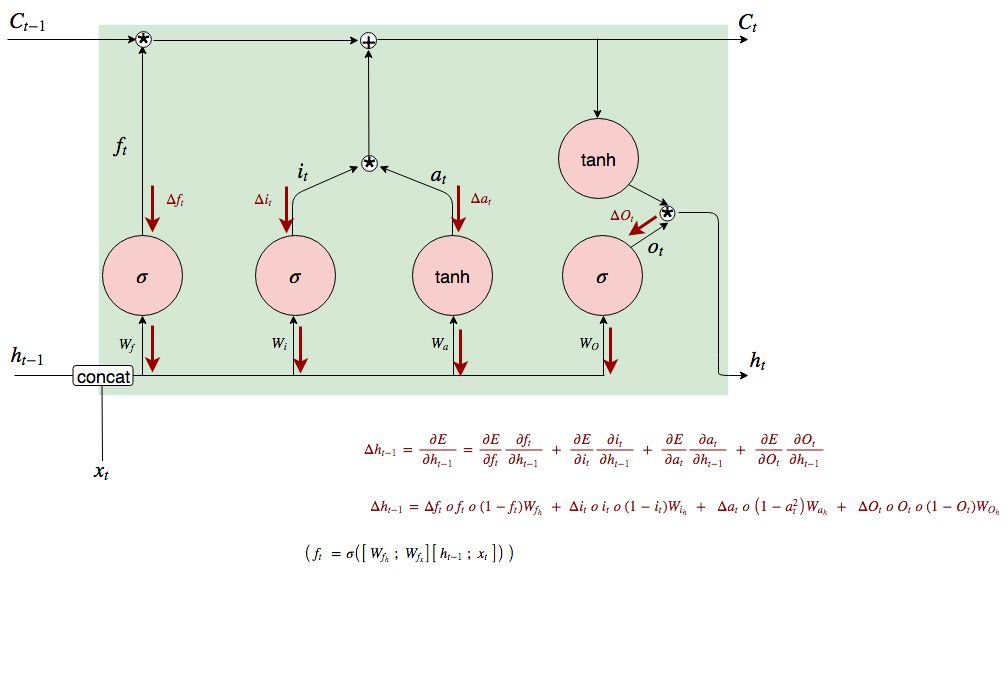
\includegraphics[width=11cm, height=8cm]{lstm_backpropagation_7.jpg}
\end{figure}
\end{frame}

\begin{frame}{Parameters update}
We have calculated $\Delta W_f$, $\Delta W_i$, $\Delta W_a$ and $\Delta W_o$. 
\\Next step is to do gradient descent:\\
$W^*$ = $W^*$ - $\alpha\Delta W^*$ where $* \in f, i, a, o
\end{frame}

\begin{frame}{References}
\begin{itemize}
    \item colah.github.io/posts/2015-08-Understanding-LSTMs
    \item www.wildml.com/2015/11/understanding-convolutional-neural-networks-for-nlp
    \item www.youtube.com/watch?v=KGOBB3wUbdc
    \item Zhang, Y., & Wallace, B. (2015). A Sensitivity Analysis of (and Practitioners’ Guide to) Convolutional Neural Networks for Sentence Classification.
    \item A Gentle Tutorial of Recurrent Neural Network with Error Backpropagation Gang Chen 
    \item www.wildml.com/2015/10/recurrent-neural-networks-tutorial-part-3-backpropagation-through-time-and-vanishing-gradients/
\end{itemize}
\end{frame}

\end{document}
